%%%%%%%%%%%%%%%%%%%%%%%%%%%%%%%%%%%%%%%%%%%%%%%%%%%%%%%%%%%%%%%%%%%%%%%%%%%%%%%%
\chapter{Проектирование аспектно-ориентированного расширения для языка Kotlin}
\label{cha:extension_design}
%%%%%%%%%%%%%%%%%%%%%%%%%%%%%%%%%%%%%%%%%%%%%%%%%%%%%%%%%%%%%%%%%%%%%%%%%%%%%%%%
Проектируемое расширение можно условно разделить на три части:
\begin{enumerate}
	\item Часть, отвечающая за анализ файлов с описанием аспектов и построения
		модели аспектов.
	\item Часть, отвечающая за построение PSI и его компиляцию в байт-код.
	\item Часть, отвечающая за внедрение аспектов в целевую программу.
\end{enumerate}
%%%%%%%%%%%%%%%%%%%%%%%%%%%%%%%%%%%%%%%%%%%%%%%%%%%%%%%%%%%%%%%%%%%%%%%%%%%%%%%%
\section{Разработка синтаксиса аспектов}
\label{sec:aspect_syntax_design}
%%%%%%%%%%%%%%%%%%%%%%%%%%%%%%%%%%%%%%%%%%%%%%%%%%%%%%%%%%%%%%%%%%%%%%%%%%%%%%%%
По результатам анализа существующих АОП-расширений можно выделить два основных
способа описания аспектов: создание классов, каждый из которых позволяет
производить вставку кода советов или же использование дополнительного синтаксиса
описания аспектов.
Для разрабатываемого прототипа был выбран второй способ, а именно, создание
отдельного синтаксиса описания аспектов, схожего с описанием классов в языке
Kotlin.

За основу разрабатываемого синтаксиса было решено взять язык описания аспектов,
используемый в фреймворке AspectJ.
Данный выбор был сделан, во-первых, из-за большой популярности данного
АОП-расширения и, во-вторых, из-за удобства и гибкости данного способа описания
аспектов.
%%%%%%%%%%%%%%%%%%%%%%%%%%%%%%%%%%%%%%%%%%%%%%%%%%%%%%%%%%%%%%%%%%%%%%%%%%%%%%%%
\subsection{Синтаксис описания аспекта}
\label{sub:custom_aspect_syntax}
%%%%%%%%%%%%%%%%%%%%%%%%%%%%%%%%%%%%%%%%%%%%%%%%%%%%%%%%%%%%%%%%%%%%%%%%%%%%%%%%
Как и в AspectJ, сквозная функциональность инкапсулируется в сущности,
называемой \textit{аспект}.
Каждый аспект имеет свой уникальный идентификатор и может содержать как описание
советов и срезов, так и переменные и функции, предназначенные для внутреннего
использование.
Описание аспекта, в целом, похоже на описание класса в языке Kotlin: оно
начинается с ключевого слова \textit{aspect}, после чего следует идентификатор
аспекта и, затем, тело аспекта, заключенное в фигурные скобки.
Пример описания аспекта с идентификатором \textit{FooAspect} приведен в листинге
~\ref{lst:custom_aspect_example}.
  \begin{lstlisting}[style={java}, label={lst:custom_aspect_example}, 
  caption={Пример описания аспекта в разрабатываемом прототипе}]
aspect FooAspect  {
  ... Тело аспекта
}
  \end{lstlisting}
%%%%%%%%%%%%%%%%%%%%%%%%%%%%%%%%%%%%%%%%%%%%%%%%%%%%%%%%%%%%%%%%%%%%%%%%%%%%%%%%
\subsection{Синтаксис описания срезов}
\label{sub:custom_pointcut_syntax}
%%%%%%%%%%%%%%%%%%%%%%%%%%%%%%%%%%%%%%%%%%%%%%%%%%%%%%%%%%%%%%%%%%%%%%%%%%%%%%%%
За основу синтаксиса описания срезов был также взят фреймворк AspectJ.
Описание среза начинается с ключевого слова \textit{pointcut}, после чего
следует идентификатор среза, уникальный в рамках данного аспекта, перечень
аргументов и, непосредственно, описание среза.
При описании среза могут использоваться следующие конструкции:
\begin{itemize}
	\item \textit{call(паттерн\_метода)} --- в срез будут добавлены все места в
		  программе, где происходит вызов метода, чей паттерн описан внутри
	  	сигнатуры.
	\item \textit{execution(паттерн\_метода)} --- в срез будут добавлены все
		  места программы, находящиеся внутри тела метода, чей паттерн описан внутри
		  сигнатуры.
	\item \textit{target(паттерн\_типа)} --- вызов метода у экземпляра, имеющего
		  тип, указанный в сигнатуре.
		  При использовании сигнатуры \textit{target} вместо типа может быть указан
		  идентификатор экземпляра класса, при условии, что данный экземпляр передан
		  в качестве агрумента при описании среза.
\end{itemize}

Описание метода также состоит из нескольких частей, описанных ниже в порядке их
следования:
\begin{enumerate}
	\item \textit{аннотации метода} --- необязательный параметр, содержащий
		  список аннотаций.
		  Можно задавать как обязательное наличие, так и отсутствие определенной
		  аннотации при помощи символа \quotes{!}.
	\item \textit{модификаторы метода} --- необязательный параметр, содержащий
		  описание модификаторов метода.
		  Может принимать следующие значения: public, private, protected,
		  internal, synchronized, final.
		  Можно задавать как обязательное наличие, так и отсутствие какого-либо
		  модификатора при помощи символа \quotes{!}.
	\item \textit{extension модификатор} --- необязательный параметр, задающий,
		  является ли функция \quotes{расширением} или нет.
	\item ключевое слово \quotes{fun}.
	\item \textit{название пакета} --- необязательный параметр, задающий имя
		  пакета и класса, в котором объявлена функция.
		  Возможен пропуск одного или нескольких символов, при помощи символа
		  \quotes{*}.
	\item \textit{имя функции} --- обязательный параметр, задающий имя функции.
		  Возможен пропуск одного или нескольких символов, при помощи символа
		  \quotes{*}.
	\item \textit{список типов параметров функции} --- необязательны параметр,
		  задающий список типов аргументов, которые имеет функция, в
		  соответствующем порядке.
		  В качестве типов, могут использоваться как стандартные типы языка
		  Kotlin, как, например, Double, Int, Short и т.д., так и
		  пользовательские типы данных.
		  Опционально можно указывать соответствие параметров функции на
		  \quotes{NotNull} и \quotes{Nullable} при помощи модификаторов
		  \quotes{!!} и \quotes{?} соответственно.
		  Если количество и типы аргументов функции не имеет значения, то это
		  можно указать, используя символ \quotes{..}.
		  Список параметров оборачивается в круглые скобки.
	\item \textit{тип возвращаемого значения} --- необязательный параметр,
		  показывающий тип значения, возвращаемого функцией.
		  В качестве типа, могут использоваться как стандартные типы языка
		  Kotlin, как, например, Double, Int, Short и т.д., так и
		  пользовательские типы данных.
		  Также как и при указании параметров функции, типу возвращаемого
		  значения можно задавать соответствие на \quotes{NotNull} и
		  \quotes{Nullable} при помощи модификаторов \quotes{!!} и \quotes{?}.
		  При указании типа возвращаемого значения, оно отделяется от списка
		  аргументов символом \quotes{:}, по аналогии с описанием функций на
		  языке Kotlin.
\end{enumerate}

Данные конструкции могут группироваться между собой при помощи следующих
логических операций \textit{конъюнкции} (\&\&),  \textit{дизъюнкции} (||)  и
\textit{инверсии} (!).
При описании срезов могут использоваться не только указанные выше сигнатуры, но
и идентификаторы других срезов, что позволяет делать описание советов более
компактным и избегать дублирования программного кода.
%%%%%%%%%%%%%%%%%%%%%%%%%%%%%%%%%%%%%%%%%%%%%%%%%%%%%%%%%%%%%%%%%%%%%%%%%%%%%%%%
\subsection{Синтаксис описания советов}
\label{sub:custom_advice_syntax}
%%%%%%%%%%%%%%%%%%%%%%%%%%%%%%%%%%%%%%%%%%%%%%%%%%%%%%%%%%%%%%%%%%%%%%%%%%%%%%%%
Описание советов также во многом схоже с описанием, используемым в AspectJ.
Оно начинается с ключевого слова, описывающего способ внедрения
кода совета относительно точки объединения, а именно:
\begin{itemize}
	\item \textit{before} --- вставка кода совета до точки объединения;
	\item \textit{after} --- вставка кода совета после точки объединения;
	\item \textit{around} --- вставка кода совета до и после точки объединения;
\end{itemize}
После этого могут следовать аргументы функций, к которым будет производиться
обращение внутри кода совета.

Следующей частью совета является описание среза, аналогичное представленному в
разделе~\ref{sub:custom_pointcut_syntax}, после которого следует код совета,
представляющий из себя программный код на языке Kotlin.
%%%%%%%%%%%%%%%%%%%%%%%%%%%%%%%%%%%%%%%%%%%%%%%%%%%%%%%%%%%%%%%%%%%%%%%%%%%%%%%%
\section{Структура программной системы}
\label{sec:prototype_structure}
%%%%%%%%%%%%%%%%%%%%%%%%%%%%%%%%%%%%%%%%%%%%%%%%%%%%%%%%%%%%%%%%%%%%%%%%%%%%%%%%
Перед проектированием структуры будущей системы, необходимо выбрать способ
внедрения аспектов.
Ввиду того, что внедрение аспектов при помощи прокси-объектов может значительно
ухудшить быстродействие системы, а при анализе байт-кода невозможно выделить
ряд специфичных для языка Kotlin языковых конструкций, было решено использовать
статический способ применения аспектов.
Внедрение аспектов сразу после компиляции является трудным в реализации, по
причинам, описанным выше.
При анализе, непосредственно, исходных кодов программы необходимо реализовывать
грамматику языка Kotlin, что также требует больших затрат.
Исходя из этих причин, было решено внедрять аспекты непосредственно в процессе
компиляции, путем модификации промежуточного представления программы.

После анализа поставленной задачи и существующих на данных момент
АОП-расширений, была предложена следующая архитектура программной системы,
представленная на рисунке~\ref{fig:program_architecture}.

\begin{figure}[htbp]
\centering
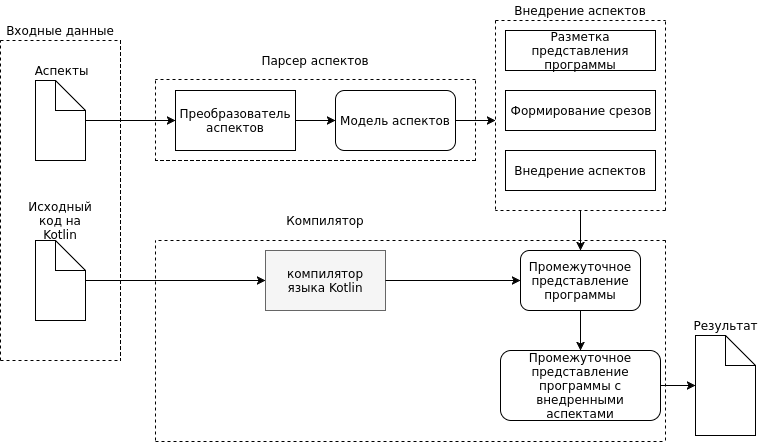
\includegraphics[width=\textwidth]{fig/program_architecture}
\caption{Архитектура программной системы}%
\label{fig:program_architecture}
\end{figure}

Как видно из рисунка~\ref{fig:program_architecture}, система состоит из
следующих частей:
\begin{enumerate}
	\item Первой частью системы являются преобразователи, отвечающие за
		 импортирование исходного кода и описания аспектов и приведения их к
		 виду промежуточного представления.
		 Для создания преобразователя аспектов, необходимо сформировать
		 грамматику описания аспектов.
		 Создание промежуточного представления программы может быть переложено
		 на компилятор языка Kotlin.
	\item Второй частью системы является часть, отвечающая за внедрение аспектов
		в промежуточное представление программы.
		Данная часть состоит из нескольких компонентов: части, отвечающей за
		разметку промежуточного представления, части, отвечающей за формирование
		срезов и части, реализующей внедрение аспектов.
	\item Последней частью системы является часть, отвечающая за компиляцию
		модифицированного промежуточного представления программы в байт-код.
		Данную часть также нет необходимости реализовывать полностью самому, так
		как можно воспользоваться готовыми системами сборки, передав в них
		не исходные коды программы, а модифицированное промежуточное
		представление.
\end{enumerate}

Таким образом, основное внимание стоит уделить модулям, отвечающим за построение
модели аспектов и внедрению аспектов в промежуточное представление программы.
%%%%%%%%%%%%%%%%%%%%%%%%%%%%%%%%%%%%%%%%%%%%%%%%%%%%%%%%%%%%%%%%%%%%%%%%%%%%%%%%
\section{Внедрение аспектов}
\label{sub:custom_aspect_weaving}
%%%%%%%%%%%%%%%%%%%%%%%%%%%%%%%%%%%%%%%%%%%%%%%%%%%%%%%%%%%%%%%%%%%%%%%%%%%%%%%%
Первая часть данного раздел посвящена описанию промежуточного представления,
создаваемому в процессе компиляции программ на Kotlin.
Во второй части будет приведено описание способа применения аспектов к PSI.
%%%%%%%%%%%%%%%%%%%%%%%%%%%%%%%%%%%%%%%%%%%%%%%%%%%%%%%%%%%%%%%%%%%%%%%%%%%%%%%%
\subsection{Описание PSI}
\label{sub:psi_description}
%%%%%%%%%%%%%%%%%%%%%%%%%%%%%%%%%%%%%%%%%%%%%%%%%%%%%%%%%%%%%%%%%%%%%%%%%%%%%%%%
\nomenclature{PSI}{Program Structure Interface}
Язык Kotlin имеет ряд оригинальных языковых конструкций (extension функции,
специфичные лямбда-функции и т.п.), при этом основной целевой платформой
компиляции для языка Kotlin является JVM.
Как результат --- все специальные конструкции Kotlin преобразуются в стандартный
байт-код, который имеет одинаковую структуру и для Java, и для Kotlin-программ.
Не смотря на то, что в версии языка Kotlin 1.1.1 часть специфичных для языка
Kotlin конструкций можно выбелить при помощи Reflection, некоторые конструкции,
как например inline функции невозможно.
%% Предложение выше неплохо бы уточнить
Из-за этого поиск некоторых структур языка Kotlin в байт-коде становится
затруднительным и, как следствие, динамическое внедрение кода советов при
загрузке файлов в JVM становится практически невозможным.
По той же причине статическое внедрение советов в байт-код программы также
является очень сложной задачей.

Таким образом, в качестве способа внедрения аспектов было выбрано внедрение аспектов в исходный код программы или в модель программы во время компиляции. 

Внедрение аспектов происходит в несколько этапов, схематически изображенных на
рисунке~\ref{fig:aspect_weaving}.
\begin{figure*}[!h]
\centering
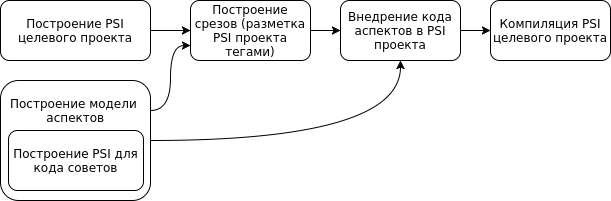
\includegraphics[width=1\textwidth]{fig/aspect_weaving}
\caption{Процесс внедрения аспектов в программный код при компиляции}
\label{fig:aspect_weaving}
\end{figure*}

Разработчики языка Kotlin предусмотрели специальную структуру данных для работы
с программным кодом --- Program Structure Interface (PSI), более.
В нашем проекте мы используем PSI для внедрения объектов на этапе компиляции
проекта.

\textit{PSI} --- промежуточное представление программного кода, используемого
разработчиками языка Kotlin при компиляции.
PSI представляет из себя набор виртуальных файлов~\cite{psi_file},
соответствующих реальным файлам с исходными кодами программы.
Каждый виртуальный файл, помимо информации о соответствующем реальном файле,
содержит дерево разбора содержимого файла, представленного в виде иерархии
объектов, типа \textit{PsiElement}~\cite{psi_element}.
Виртуальный файл также является наследником интерфейса PsiElement.
%%%%%%%%%%%%%%%%%%%%%%%%%%%%%%%%%%%%%%%%%%%%%%%%%%%%%%%%%%%%%%%%%%%%%%%%%%%%%%%%
\subsubsection{Интерфейс PsiElement}
\label{ssub:psi_element_description}
%%%%%%%%%%%%%%%%%%%%%%%%%%%%%%%%%%%%%%%%%%%%%%%%%%%%%%%%%%%%%%%%%%%%%%%%%%%%%%%%
Интерфейс PsiElement является базовым интерфейсом, от которого унаследованы все
элементы, являющиеся узлами PSI.
Он содержит множество функций для манипуляций с PSI, однако, при проектировании
АОП-расширения, нас, в первую очередь, интересуют следующее:
\begin{itemize}
	\item \textit{Project getProject()} --- метод, возвращающий проект, к
		которому относится данный элемент.
	\item \textit{PsiElement[] getChildren()} --- метод, возвращающий список
		дочерних элементов данного элемента.
	\item \textit{PsiElement getParent()} --- метод, возвращающий родительский
		элемент.
	\item \textit{String getText()} --- метод, возвращающий текстовое
		представление элемента.
	\item \textit{PsiElement copy()} --- метод, возвращающий копию данного
		элемента.
	\item \textit{PsiElement add(@NotNull PsiElement element) throws
		IncorrectOperationException} --- метод, позволяющий добавлять потомка
		\textit{element} к данному элементу.
		Данный метод возвращает фактически добавленный элемент или его копию.
	\item \textit{PsiElement addBefore(@NotNull PsiElement element, @Nullable
		PsiElement anchor) throws IncorrectOperationException} --- метод,
		позволяющий добавлять элемент \textit{element} перед элементом
		\textit{anchor}.
		Данный метод возвращает фактически добавленный элемент или его копию.
	\item \textit{PsiElement addAfter(@NotNull PsiElement element, @Nullable
		PsiElement anchor) throws IncorrectOperationException} --- метод,
		позволяющий добавлять элемент \textit{element} после элемента
		\textit{anchor}.
		Данный метод возвращает фактически добавленный элемент или его копию.
	\item \textit{void checkAdd(@NotNull PsiElement element) throws
		IncorrectOperationException} --- метод, проверяющий возможность
		добавления потомка \textit{element} к текущему элементу.
		В случае, если операция невозможна по каким-либо причинам, выбрасывается
		исключение \textit{IncorrectOperationException}.
	\item \textit{PsiElement replace(@NotNull PsiElement newElement) throws
		IncorrectOperationException} --- метод, позволяющий заменять текущий
		элемент, элементом \textit{newElement}.
		Данный метод возвращает элемент, который был добавлен в дерево.
	\item \textit{<T> T getCopyableUserData(Key<T> key)} --- метод, возвращающий
		пользовательские данные, находящиеся в структуре \textit{myUserData}
		с ключем \textit{key}.
	\item \textit{<T> void putCopyableUserData(Key<T> key, @Nullable T value)}
		--- метод, позволяющий сохранить пользовательские данные
		\textit{value}, в структуре \textit{myUserData} под ключем \textit{key}.
\end{itemize}
%%%%%%%%%%%%%%%%%%%%%%%%%%%%%%%%%%%%%%%%%%%%%%%%%%%%%%%%%%%%%%%%%%%%%%%%%%%%%%%%
\subsubsection{Класс KtCallExpression}
\label{ssub:kt_call_expression_description}
%%%%%%%%%%%%%%%%%%%%%%%%%%%%%%%%%%%%%%%%%%%%%%%%%%%%%%%%%%%%%%%%%%%%%%%%%%%%%%%%
Класс \textit{KtCallExpression} представляет узел, соответствующий вызову
функции.
В разрабатываемом расширении предполагается использовать следующие методы
данного класса:
\begin{itemize}
	\item \textit{getResolvedCall(context: BindingContext): ResolvedCall
		<CallableDescriptor>?} --- метод, позволяющий получать дескриптор
		вызываемой функции.
\end{itemize}
%%%%%%%%%%%%%%%%%%%%%%%%%%%%%%%%%%%%%%%%%%%%%%%%%%%%%%%%%%%%%%%%%%%%%%%%%%%%%%%%
\subsubsection{Класс KtNamedFunction}
\label{ssub:kt_named_function_description}
%%%%%%%%%%%%%%%%%%%%%%%%%%%%%%%%%%%%%%%%%%%%%%%%%%%%%%%%%%%%%%%%%%%%%%%%%%%%%%%%
Класс \textit{KtNamedFunction} представляет узел, соответствующий объявлению
именованной функции.
В разрабатываемом расширении предполагается использовать следующие методы
данного класса:
\begin{itemize}
	\item \textit{getResolvedCall(context: BindingContext): ResolvedCall
		<CallableDescriptor>?} --- метод, позволяющий получать дескриптор
		вызываемой функции.
	\item \textit{getValueParameters(): MutableList<KtParameter>} --- метод,
		позволяющий получить список аргументов, принимаемых функцией в виде
		списка элементов типа \textit{KtParameter}.
	\item \textit{hasDeclaredReturnType(): Boolean} --- метод, позволяющий
		узнать, возвращает ли функция какое-либо значение или нет.
	\item \textit{getTypeReference(): KtTypeReference?} --- метод, позволяющий
		получить тип возвращаемого функцией значения.
	\item \textit{isExtensionDeclaration(): Boolean} --- метод, позволяющий
		проверить является ли данная функция extension или нет.
	\item \textit{isPrivate(): Boolean} --- метод, позволяющий проверить,
		является ли данная функция приватной.
	\item \textit{isProtected(): Boolean} --- метод, позволяющий проверить,
		является ли данная функция protected.
	\item \textit{getModifierList(): KtModifierList?} --- метод, позволяющий
		получить список модификаторов функции.
		Данный метод возвращает экземпляр класса \textit{KtModifierList}, содержащий
		в списке узлов модификаторы функции.
\end{itemize}
%%%%%%%%%%%%%%%%%%%%%%%%%%%%%%%%%%%%%%%%%%%%%%%%%%%%%%%%%%%%%%%%%%%%%%%%%%%%%%%%
\subsubsection{CallableDescriptor}
\label{ssub:callable_descriptor_description}
%%%%%%%%%%%%%%%%%%%%%%%%%%%%%%%%%%%%%%%%%%%%%%%%%%%%%%%%%%%%%%%%%%%%%%%%%%%%%%%%
Класс \textit{CallableDescriptor} представляет узел, соответствующий
дескриптору вызываемой функции.
В разрабатываемом расширении предполагается использовать следующие методы
данного класса:
\begin{itemize}
	\item \textit{getName(): Name} --- метод, возвращающий имя функции в виде
		экземпляра типа \textit{Name}.
	\item \textit{getExtensionReceiverParameter(): ReceiverParameterDescriptor}
		--- метод, позволяющий получить имя класса и пакета, к которому принадлежит
		 extension функция.
	\item \textit{getContainingDeclaration(): DeclarationDescriptor} --- метод,
		позволяющий получить имя класса и пакета, к которому принадлежит не
		extension функция.
	\item \textit{getValueParameters(): MutableList<ValueParameterDescriptorImpl>}
		--- метод, позволяющий получить список аргументов, принимаемых функцией в
		виде списка элементов типа \textit{ValueParameterDescriptorImpl}.
	\item \textit{getReturnType(): KotlinType?} --- метод, позволяющий получить
		тип возвращаемого функцией значения.
	\item \textit{isExtension(): Boolean} --- метод, позволяющий проверить
		является ли данная функция extension или нет.
	\item \textit{isInline(): Boolean} --- метод, позволяющий проверить
		является ли данная функция inline или нет.
	\item \textit{getVisibility(): Visibility} --- метод, позволяющий получить
		класс, содержащий в себе видимость функции (является ли функция
		\textit{public}, или \textit{private}, или \textit{protected}).
\end{itemize}
%%%%%%%%%%%%%%%%%%%%%%%%%%%%%%%%%%%%%%%%%%%%%%%%%%%%%%%%%%%%%%%%%%%%%%%%%%%%%%%%
\subsection{Формирование срезов}
\label{ssec:pointcut_creation_description}
%%%%%%%%%%%%%%%%%%%%%%%%%%%%%%%%%%%%%%%%%%%%%%%%%%%%%%%%%%%%%%%%%%%%%%%%%%%%%%%%
При формировании срезов, каждый узел PSI проверяется на соответствие тому или
иному срезу.
При рассмотрении принадлежности узла PSI к срезу происходит в несколько шагов.
Первым шагом является выбор всех терминальных узлов в описании среза.
В случае, если каким-либо из терминальных узлов является идентификатор другого
среза, необходимо вычислить принадлежность узла к этому срезу.
Следующим шагом для каждого для каждого терминального узла производится
проверка на то, какие из узлов PSI ему соответствуют.
При соответствии узла PSI терминальному узлу описания среза, в структуру
<<userMap>> данного узла помещается идентификатор данного узла.
Последним шагом является вычисление логического выражения для каждого из узлов
PSI.
ПРи вычислении значения логического выражения, для каждого из терминальных узлов
подставляется \textit{True}, если узел PSI содержит идентификатор данного узла
и \textit{False}, если нет.
В случает, если логическое выражение истино, в структуру \textit{userMap}
добавляется идентификатор среза.
После чего анализ переходит к следующему узлу PSI.

%%%%%%%%%%%%%%%%%%%%%%%%%%%%%%%%%%%%%%%%%%%%%%%%%%%%%%%%%%%%%%%%%%%%%%%%%%%%%%%%
\subsubsection{Сигнатура \textit{call}}
\label{ssub:call_signature_mark}
%%%%%%%%%%%%%%%%%%%%%%%%%%%%%%%%%%%%%%%%%%%%%%%%%%%%%%%%%%%%%%%%%%%%%%%%%%%%%%%%
Для поиска всех потенциальных точек программы, которые могут соответствовать
данной сигнатуре, необходимо выбрать все узлы PSI, имеющие тип
\textit{KtCallExpression} (подробно данный класс описан в разделе
\ref{ssub:kt_call_expression_description}) --- тип, представляющий места вызова
функций в PSI.

После того, как выбраны все узлы, соответствующие вызовам функции необходимо
получить дескриптор вызываемой функции для того, чтобы проверить соответствие
вызываемой функции описанию внутри сигнатуры.
Для того, что бы получить дескриптор, можно воспользоваться методом
\textit{getResolvedCall}, позволяющий получить дескриптор вызываемого метода.
Из данного дескриптора можно получить следующие свойства функции:
\begin{itemize}
	\item Имя функции, при помощи property \textit{name}.
	\item Класс и пакет, к которому относится функция.
		  	В случае, если рассматриваемый метод является extension декларацией,
		  	класс ,которой она расширяет можно получить при помощи property
		  	\textit{extensionReceiverParameter}.
		  	В противном случае, название класса и пакета можно получить при помощи
		  	property \textit{fqNameSafe}.
	\item Список параметров, передаваемых по значению при помощи property
		 	  \textit{valueParameters}.
				О каждом параметра, в свою очередь можно получить следующую информацию:
	\begin{itemize}
		\item Тип, при помощи property \textit{type}
		\item Nullability модификатор при помощи метода \textit{isMarkedNullable()}
	\end{itemize}
	\item Возвращаемое функцией значение при помощи property \textit{returnType}
	\item Является ли рассматриваемый метод extension декларацией, при помощи
				метода isExtension(), возвращающий true в случае, если рассматриваемая
				функция является extension и false в противном случае.
	\item Является ли рассматриваемый метод inline функцией, при помощи метода
				isInline(), возвращающий true в случае, если рассматриваемая функция
				является inline и false в противном случае.
	\item Видимость метода при помощи property \textit{visibility}
\end{itemize}
При проверке соответствия каждого из параметров функции сигнатуре метода необходимо учитывать, что любой из параметров в сигнатуре может иметь знак инверсии.
В случае наличия в сигнатуре знака отрицания, необходимо инвертировать результат сравнения.

В случае, если дескриптор метода полностью совпадает с маской метода внутри
сигнатуры \textit{call}, в структуру \textit{myUserData} данного узла PSI
помещается идентификатор сигнатуры.
%%%%%%%%%%%%%%%%%%%%%%%%%%%%%%%%%%%%%%%%%%%%%%%%%%%%%%%%%%%%%%%%%%%%%%%%%%%%%%%%
\subsubsection{Сигнатура \textit{execution}}
\label{ssub:execution_signature}
%%%%%%%%%%%%%%%%%%%%%%%%%%%%%%%%%%%%%%%%%%%%%%%%%%%%%%%%%%%%%%%%%%%%%%%%%%%%%%%%
Для поиска всех мест, где объявлены именованные функции, необходимо выбрать все
узлы PSI, реализующие класс \textit{KtNamedFunction} (подробно данный класс
описан в разделе \ref{ssub:kt_named_function_description}).

После чего из каждого экземпляра данного класса можно получить следующие параметры метода:
\begin{itemize}
	\item Имя метода, при помощи property \textit{name}
	\item Название класса и пакета, к которому принадлежит метод.
				В случае, если метод является execution декларацией, класс, который он
				расширяет можно получить из property \textit{receiverTypeReference}.
				В противном случае класс, внутри которого объявлен метод можно получить
				при	помощи property \textit{containingClassOrObject} (в случае, если
				метод не принадлежит ни к какому классу, property вернет значение null).
	\item Тип возвращаемого методом значения, при помощи property
				\textit{typeReference}
	\item Список параметров, принимаемых по значению при помощи property
				\textit{valueParameters}
	\item Является ли метод execution декларацией класса при помощи метода
				\textit{isExtensionDeclaration()}
	\item Список модификаторов метода при помощи property \textit{modifierList}
	\item Является ли функция приватной, при помощи метода \textit{isPrivate()}
	\item Является ли функция protected, при помощи метода \textit{isProtected()}
\end{itemize}

Как и в случае с сигнатурой \textit{call}, каждый из параметров в маске может
иметь знак инверсии, что необходимо учитывать при сравнении метода с сигнатурой.

В случае, если данный метод попадает под маску, заданную в сигнатуре, то
необходимо поместить идентификатор во все узлы, находящиеся в теле функции.
Тело функции можно получить при помощи property \textit{bodyExpression}.
%%%%%%%%%%%%%%%%%%%%%%%%%%%%%%%%%%%%%%%%%%%%%%%%%%%%%%%%%%%%%%%%%%%%%%%%%%%%%%%%
\subsubsection{Сигнатура \textit{target}}
\label{ssub:target_signature}
%%%%%%%%%%%%%%%%%%%%%%%%%%%%%%%%%%%%%%%%%%%%%%%%%%%%%%%%%%%%%%%%%%%%%%%%%%%%%%%%
Для поиска всех потенциальных точек программы, которые могут соответствовать
данной сигнатуре, необходимо выбрать все узлы PSI, имеющие тип
\textit{KtCallExpression} (подробно данный класс описан в разделе
\ref{ssub:kt_call_expression_description}) --- тип, представляющий места вызова
функций в PSI.
После чего, как и в случае с сигнатурой \textit{call}, необходимо получить
дескриптор метода при помощи метода \textit{getResolvedCall} и затем класс, на
экземпляре которого вызывается данный метод при помощи property
\textit{extensionReceiverParameter} в случае, если метод является execution
декларацией.
В противном случае, название класса и пакета можно получить при помощи property
\textit{fqNameSafe}.

Если полученный тип удовлет	типу, описанному в сигнатуре, то в структуру
\textit{myUserData} рассматриваемого элемента помещается идентификатор
сигнатуры.
%%%%%%%%%%%%%%%%%%%%%%%%%%%%%%%%%%%%%%%%%%%%%%%%%%%%%%%%%%%%%%%%%%%%%%%%%%%%%%%%
\subsection{Внедрение кода советов}
\label{sub:advice_applying_description}
%%%%%%%%%%%%%%%%%%%%%%%%%%%%%%%%%%%%%%%%%%%%%%%%%%%%%%%%%%%%%%%%%%%%%%%%%%%%%%%%
В общем случае применение кода совета сводится к внедрению конвертированного в
PSI кода совета в PSI проекта.
Однако, в случае применения кода совета к функции может возникнуть ситуация,
когда результат, возвращаемый функцией сразу же используется далее.

Для наглядности, рассмотрим участок кода, приведенный в листинге
\ref{lst:target_ex}:
\begin{lstlisting}[style={java}, label=lst:target_ex,
    caption={Пример целевой точки внедрения}]
...
val res = A.foo().bar().baz()
...
\end{lstlisting}
Допустим, что нам нужно применить код совета, сразу после вызова метода
\textit{foo}.
Одним из стандартных способов решения данной задачи является разнесение вызовов
функций, представленный в листинге \ref{lst:standart_decomp_ex}:
\begin{lstlisting}[style={java}, label=lst:standart_decomp_ex,
    caption={Пример разнесения вызовов методов}]
...
val fooRes = A.foo()
val barRes = fooRes.bar()
val res = barRes.baz()
...
\end{lstlisting}

Такой подход позволяет достаточно легко разрешать большинство последовательных
вызовов функций, но ситуация значительно усложняется в случае, если, например,
последовательный вызов функций является аргументов какой-либо другой функции.
В качестве примера рассмотрим участок программного кода, приведенный в листинге
\ref{lst:target_in_argument_ex}:
\begin{lstlisting}[style={java}, label=lst:target_in_argument_ex,
    caption={Пример целевой точки внедрения, передаваемой в качестве аргумента другому методу}]
...
val res = quux(A.foo().bar().baz())
...
\end{lstlisting}
В таком случае, необходимо произвести разнесение аргументов вне функции
\textit{quux}, а после чего передать последний из результатов вычислений в
качестве аргумента.
При этом модифицированный код программы был бы приведен к виду, представленному
в листинге \ref{lst:standart_decomp_args_ex}.
\begin{lstlisting}[style={java}, label=lst:standart_decomp_args_ex,
    caption={Пример разнесения вызовов методов, переданных в качестве аргументов}]
...
val fooRes = A.foo()
val barRes = fooRes.bar()
val bazRes = barRes.baz()
val res = quux(bazRes)
...
\end{lstlisting}

Такое разнесение вызовов функций является достаточно трудоемкой задачей, как
при модификации исходных кодов, так и промежуточного представления.
Для того, чтобы сделать внедрение кода советов более удобным, было решено
оборачивать точку внедрения в лябда-враппер \textit{run}.
При этом результат работы функции также как и в ситуации выше присваивается
промежуточной переменной.
Данная переменная имеет область видимости в пределах потока управления
лямбда-враппера и не видна извне.
Снаружи такая конструкция выглядит как единая функция, из-за чего нет
необходимости разносить вызовы функций, как это было приведено в листингах
\ref{lst:standart_decomp_ex} и \ref{lst:standart_decomp_args_ex}.

Для наглядности еще раз рассмотрим пример, приведенный в листинге
\ref{lst:target_ex}.
Допустим, нам необходимо вставить код совета после вызова метода \textit{foo}.
Для этого необходимо обернуть место вызова метода \textit{foo} в лямбда-функцию
\textit{run}.
После этого, необходимо сохранить результат, возвращенный функцией \textit{foo}
в промежуточную переменную, объявленную внутри враппера.
Следующим шагом является вставка кода совета после вызова функции \textit{foo} и возвращение сохраненного результата из функции \textit{run}.
Результат преобразования представлен в листинге~\ref{lst:apply_advice_with_run_ex}.
\begin{lstlisting}[style={java}, label=lst:apply_advice_with_run_ex,
    caption={Пример внедрения кода совета с использованием функции run}]
...
val res = A.foo().run{
        val buf = bar()
        //advice code
        buf
    }.baz()
...
\end{lstlisting}

При таком подходе отпадает необходимость разносить вызовы методов, что
значительно упрощает вставку кода совета, особенно если точка объединения
является, например, аргументом функции.

В случае, если код совета вставляется только перед вызовом функции, результат
работы функции можно не сохранять в промежуточной переменной, а возвращать
непосредственно из функции \textit{run}.
В таком случае, применение совета будет иметь вид, аналогичный представленному
в листинге \ref{lst:apply_advice_before_with_run_ex}.
\begin{lstlisting}[style={java}, label=lst:apply_advice_before_with_run_ex,
    caption={Пример внедрения кода совета после точки объединения с использованием функции run}]
...
val res = A.foo().run{
        //advice code
        bar()
    }.baz()
...
\end{lstlisting}

При перенесении элемента PSI внутрь лямбда-враппера, происходит копирование
элемента, при котором теряется информация, записанная в структуре
\textit{myUserData}.
Из-за этого, после перенесения точки внедрения внутрь враппера необходимо
обновлять теги срезов, так как к одной точке внедрения может быть применено
несколько советов.
Благодаря тому, что мы знаем размер и структуру вставляемого кода совета, а
также его место относительно точки внедрения, мы легко можем вычислить
местонахождение точки внедрения внутри функции \textit{run} и назначить ей
метки, заданные до модификации.

Возможность обращения к параметрам точки внедрения, а также к объектам, на
которых производится вызов методов, было решено оборачивать код совета в метод,
вызываемый внутри враппера \textit{run}.
В случае, если в срезе есть сигнатура \textit{target}, в качестве первого параметра метод принимает в качестве аргумента элемент, на котором происходит вызов метода.
%%TODO args
В противном случае, метод не принимает никаких аргументов.

В качестве примера рассмотрим участок кода, приведенный в листинге
\ref{lst:target_advice_pointcut_example}:
\begin{lstlisting}[style={java}, label=lst:target_advice_pointcut_example,
    caption={Пример точки внедрения}]
...
val foo = Foo()
foo.bar()
...
\end{lstlisting}
Если для среза, в который попадает вызов метода \textit{bar()} определена
сигнатура \textit{target} с переданным в неё типом \textit{Foo}, то переменная
\textit{foo} будет передана внутрь метода-обёртки.
Пример преобразования кода после применения совета приведен в листинге
\ref{lst:target_advice_weaving_example}:
\begin{lstlisting}[style={java}, label=lst:target_advice_weaving_example,
    caption={Пример применения совета, имеющего сигнатуру \textit{target}}]
...
val foo = Foo()
foo.run{
	fun adFun(f: Foo) {
		//advice code
	}
	adFun(foo)
	bar()
}
...
\end{lstlisting}

%%%%%%%%%%%%%%%%%%%%%%%%%%%%%%%%%%%%%%%%%%%%%%%%%%%%%%%%%%%%%%%%%%%%%%%%%%%%%%%%
\section{Выводы}
\label{sec:design_conclusion}
%%%%%%%%%%%%%%%%%%%%%%%%%%%%%%%%%%%%%%%%%%%%%%%%%%%%%%%%%%%%%%%%%%%%%%%%%%%%%%%%
В результате был разработан синтаксис описания аспектов для языка Kotlin,
описан способ применения аспектов, а также разработана архитектура прототипа.
Вся программная система разбита на две составляющие:
\begin{enumerate}
	\item Часть, отвечающая за формирование грамматики аспектов.
	\item Часть, отвечающая за применение аспектов к целевой программе, которая может быть разбита на две подгруппы:
	\begin{enumerate}
		\item Подгруппа, отвечающая за построение модели описанных аспектов.
		\item Подгруппа, отвечающая за внедрение аспектов в целевую программу.
	\end{enumerate}
\end{enumerate}
%%%%%%%%%%%%%%%%%%%%%%%%%%%%%%%%%%%%%%%%%%%%%%%%%%%%%%%%%%%%%%%%%%%%%%%%%%%%%%%%
